\documentclass[xetex,mathserif,serif]{beamer}
\usepackage{polyglossia}
\setdefaultlanguage[babelshorthands=true]{russian}
\usepackage{minted}
\usepackage{tabu}
\usepackage[11pt]{moresize}

\usepackage{textpos}
\setlength{\TPHorizModule}{1cm}
\setlength{\TPVertModule}{1cm}

\useoutertheme{infolines}

\usepackage{fontspec}
\setmainfont{FreeSans}
\newfontfamily{\russianfonttt}{FreeSans}

\tabulinesep=0.7mm

\newcommand{\attribution}[1] {
    \begin{flushright}\begin{scriptsize}\textcolor{gray}{\textcopyright\; #1}\end{scriptsize}\end{flushright}
}

\title{Лекция 14: Проектирование распределённых приложений (3)}
\subtitle{Стратегические вопросы}
\author[Юрий Литвинов]{Юрий Литвинов\\\small{\textcolor{gray}{yurii.litvinov@gmail.com}}}

\date{25.04.2022}

\begin{document}

    \frame{\titlepage}

    \section{Архитектурные стили распределённых систем}

    % Источник: https://github.com/MicrosoftDocs/architecture-center/tree/main/docs/guide/architecture-styles

    \begin{frame}
        \frametitle{Big Compute}
        \begin{center}
            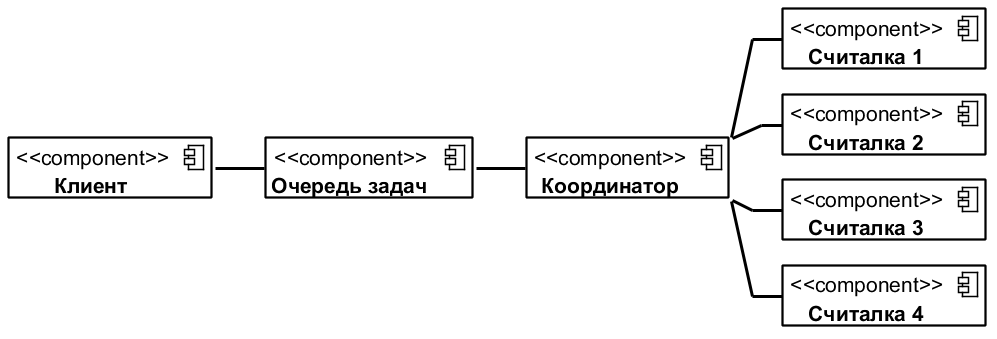
\includegraphics[width=0.8\textwidth]{bigCompute.png}
        \end{center}
        \begin{itemize}
            \item Для сверхсложных задач, предполагающих тысячи вычислительных узлов
            \item Требует <<embarrassingly parallel>> задачу
            \item Предполагает использование весьма продвинутых (и дорогих) облачных ресурсов
        \end{itemize}
    \end{frame}

    \begin{frame}
        \frametitle{Big Data}
        \begin{center}
            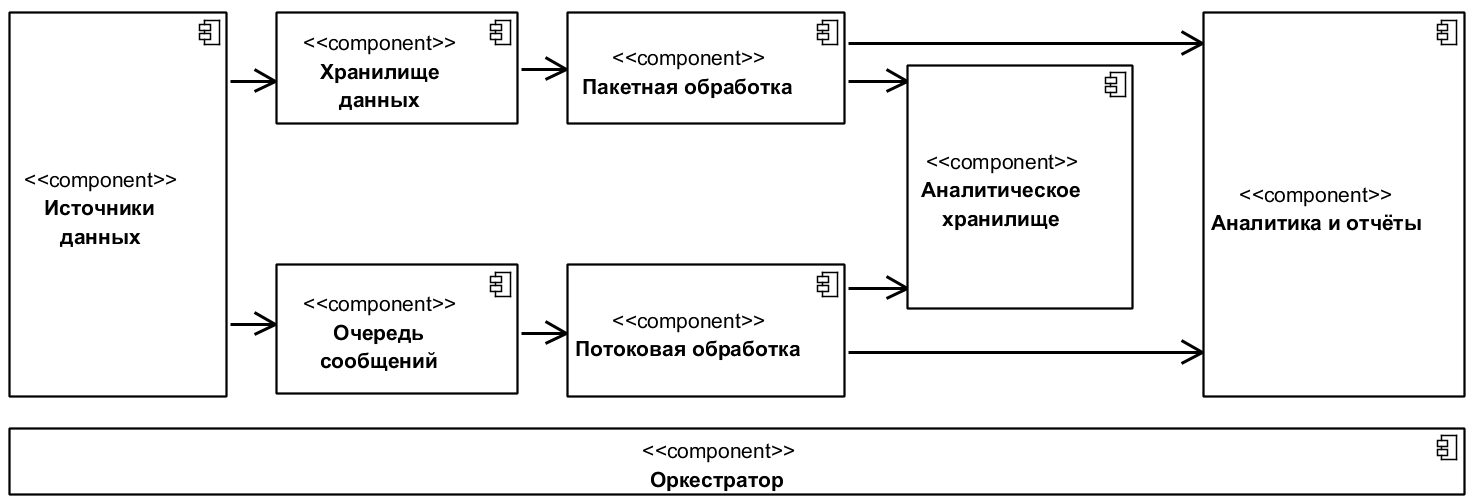
\includegraphics[width=0.9\textwidth]{bigData.png}
        \end{center}
        \begin{itemize}
            \item Для аналитики над большими данными
            \begin{itemize}
                \item Либо данных много и их можно обрабатывать неторопливо
                \item Либо данных много и их надо обрабатывать в реальном времени
            \end{itemize}
            \item Данные не лезут в обычную СУБД
        \end{itemize}
    \end{frame}

    \begin{frame}
        \frametitle{Big Data, хорошие практики}
        \begin{itemize}
            \item Распределённые хранение и обработка
            \begin{itemize}
                \item Например, Apache Hadoop, Apache Spark
            \end{itemize}
            \item Schema-on-read
            \begin{itemize}
                \item Data lake --- распределённое хранилище слабоструктурированных данных
            \end{itemize}
            \item Обработка на месте (TEL вместо ETL)
            \item Разделение данных по интервалам обработки
            \item Раннее удаление приватных данных
        \end{itemize}
    \end{frame}

    \begin{frame}
        \frametitle{Пример: IoT}
        \begin{center}
            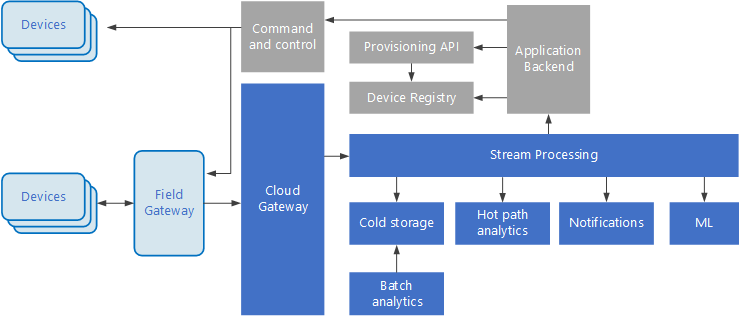
\includegraphics[width=0.9\textwidth]{iot.png}
            \attribution{https://github.com/MicrosoftDocs/architecture-center/blob/main/docs/guide/architecture-styles/big-data.md}
        \end{center}
    \end{frame}

    \begin{frame}
        \frametitle{Событийно-ориентированная архитектура}
        \begin{center}
            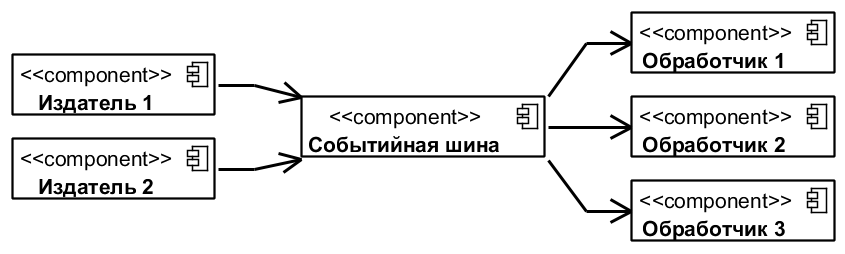
\includegraphics[width=0.7\textwidth]{eventDrivenArchitecture.png}
        \end{center}
        \begin{itemize}
            \item Для обработки событий в реальном времени
            \item Бывает двух видов:
            \begin{itemize}
                \item Издатель/подписчик (например, RabbitMQ)
                \item Event Sourcing (например, Apache Kafka)
            \end{itemize}
        \end{itemize}
    \end{frame}

    \begin{frame}
        \frametitle{Web-queue-worker}
        \begin{center}
            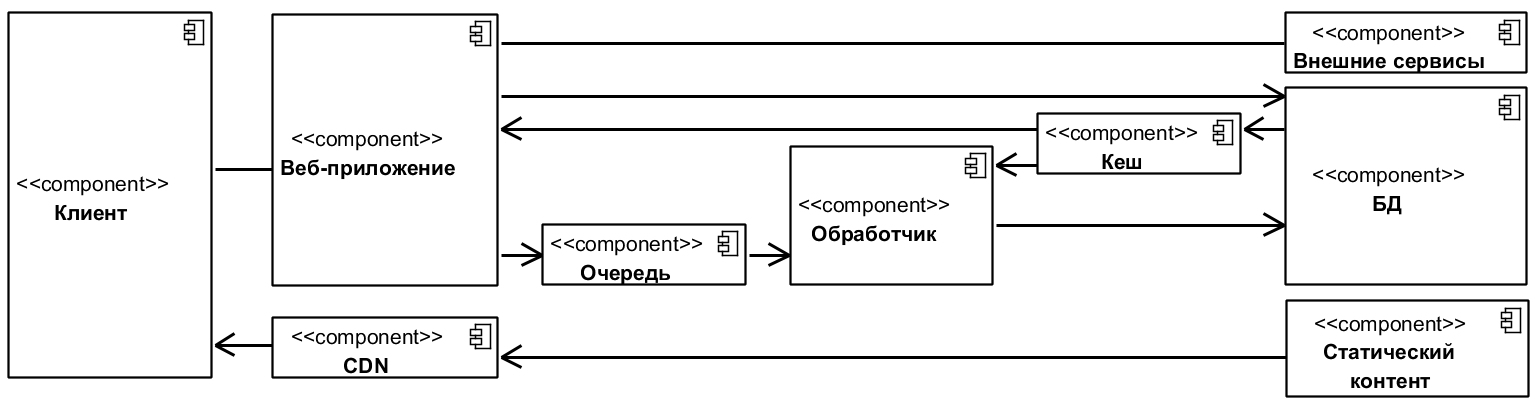
\includegraphics[width=0.9\textwidth]{webQueueWorker.png}
        \end{center}
        \begin{itemize}
            \item Для вычислительно сложных задач в несложной предметной области
            \item Позволяет эффективно использовать готовые сервисы
            \item Независимое масштабирование фронтенда и обработчика
            \item Может превратиться в Big Ball of Mud
        \end{itemize}
    \end{frame}

    \begin{frame}
        \frametitle{N-звенная архитектура}
        \begin{center}
            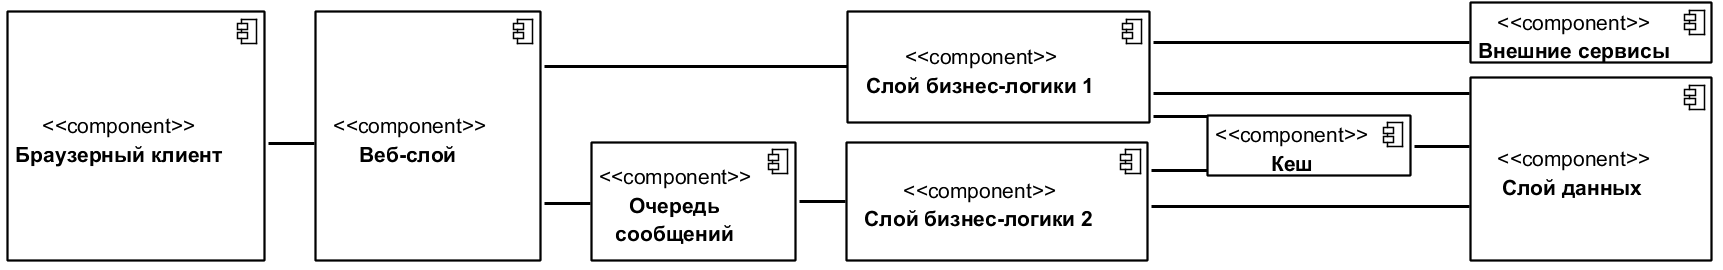
\includegraphics[width=0.9\textwidth]{nTierArchitecture.png}
        \end{center}
        \begin{itemize}
            \item Для быстрого переноса монолита в облако
            \item Для простых веб-приложений
            \item Проблемы с масштабированием и сопровождаемостью
        \end{itemize}
    \end{frame}

    \begin{frame}
        \frametitle{Пример: N-звенное приложение на Azure}
        \begin{center}
            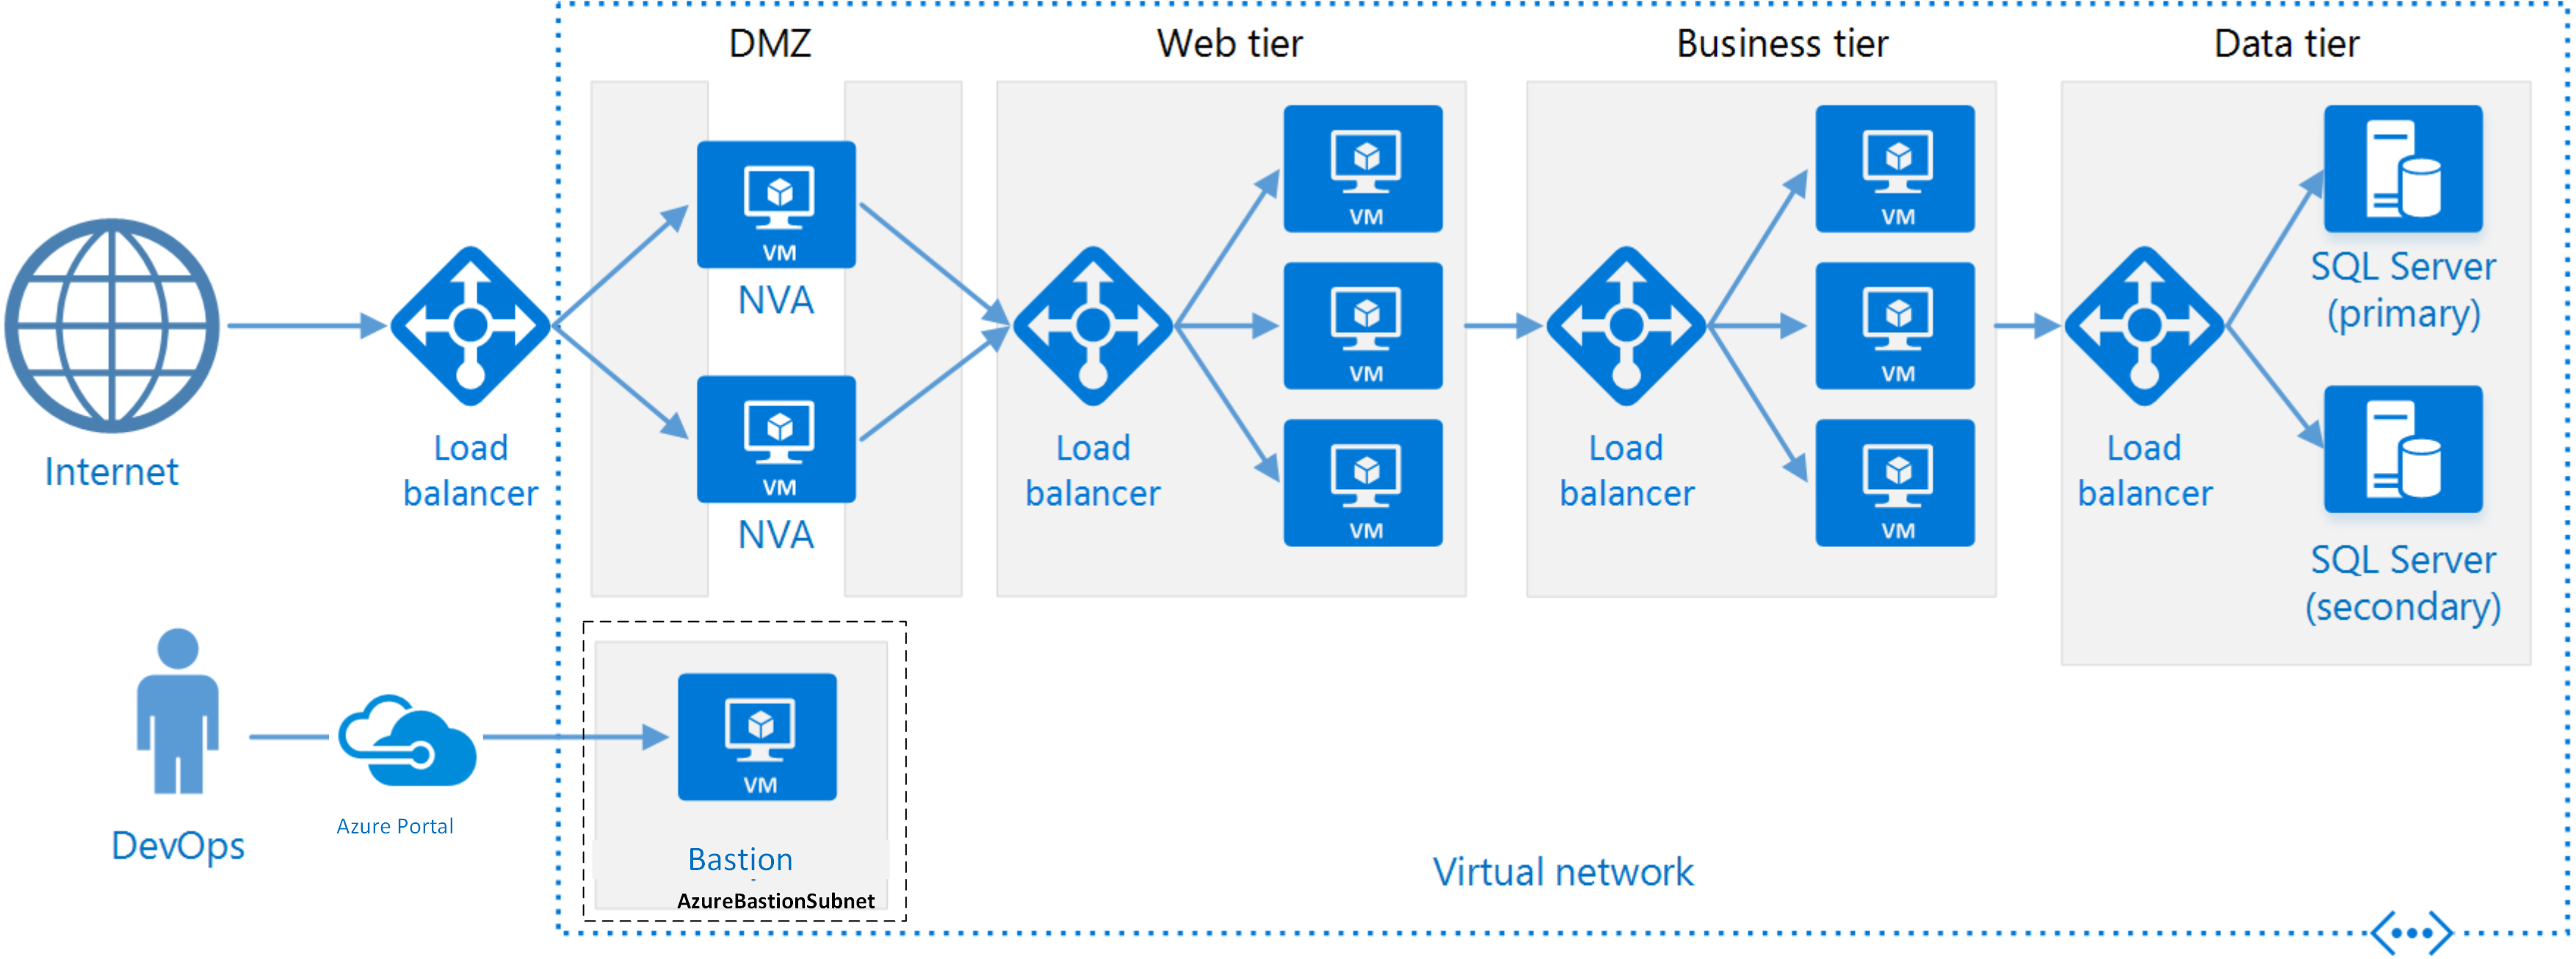
\includegraphics[width=\textwidth]{nTierAzure.png}
            \attribution{https://github.com/MicrosoftDocs/architecture-center/blob/main/docs/guide/architecture-styles/n-tier.md}
        \end{center}
    \end{frame}

    \begin{frame}
        \frametitle{Микросервисная архитектура}
        \begin{center}
            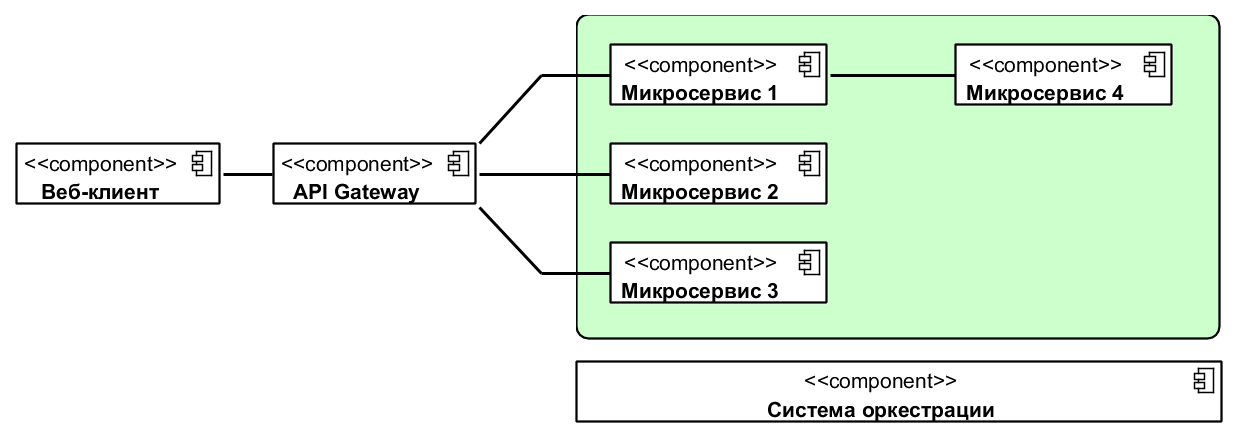
\includegraphics[width=0.85\textwidth]{microservices.png}
        \end{center}
        \begin{itemize}
            \item Для приложений со сложной предметной областью
            \item Альтернатива монолиту, со своими достоинствами и недостатками
            \item Микросервис пишется одним человеком за две недели
            \begin{itemize}
                \item На самом деле, пишется и поддерживается небольшой командой
            \end{itemize}
            \item Микросервис --- ограниченный контекст в смысле DDD
        \end{itemize}
    \end{frame}

    \section{Тактическая архитектура}

    \begin{frame}
        \frametitle{Гексагональная архитектура}
        \framesubtitle{``Порты и адаптеры''}
        \begin{columns}
            \begin{column}{0.5\textwidth}
                \begin{itemize}
                    \item Другая точка зрения на уровни: самый нижний --- уровень предметной области
                    \item Всё остальное поставляется ему как внешние зависимости
                    \item Активно используется Dependency Inversion
                    \item Порт --- по сути, интерфейс, предоставляемый или потребляемый
                    \item Адаптер --- паттерн ``Адаптер'' для ``подгонки'' интерфейсов
                \end{itemize}
            \end{column}
            \begin{column}{0.5\textwidth}
                \begin{center}
                    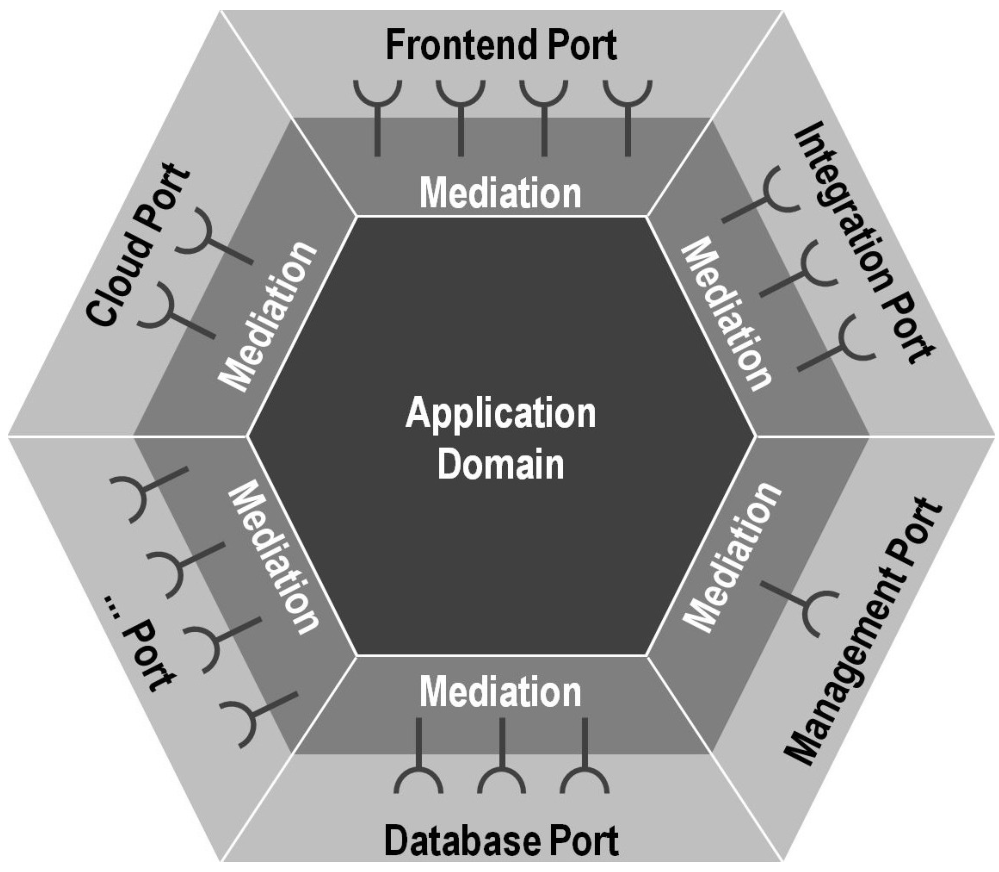
\includegraphics[width=0.8\textwidth]{hexagonalArchitecture.png}
                    \attribution{B Butzin et al, Microservices Approach for the Internet of Things}
                \end{center}
            \end{column}
        \end{columns}
    \end{frame}

    \begin{frame}
        \frametitle{Плюсы и минусы}
        Плюсы:
        \begin{itemize}
            \item Изоляция механизмов доставки
            \item Изоляция вспомогательных механизмов
            \item Лёгкость тестирования, моки
            \item Чистая бизнес-логика и модель предметной области
            \begin{itemize}
                \item Максимальная простота
                \item Возможность валидации и конвертирования данных
            \end{itemize}
        \end{itemize}
        \vspace{5mm}
        Минусы:
        \begin{itemize}
            \item Довольно тяжеловесна
            \item Непонятно, что делать с фреймворками
            \item Не очень подробна
        \end{itemize}
    \end{frame}

    \begin{frame}
        \frametitle{Луковая архитектура}
        \begin{columns}
            \begin{column}{0.5\textwidth}
                \begin{itemize}
                    \item Дальнейшее развитие гексагональной --- определяет внутреннюю структуру ядра
                    \item Внутренние слои не знают о внешних, доменная модель вообще ни о ком не знает
                    \item Внутренние слои определяют интерфейсы, внешние их реализуют
                    \item Уровневость нестрогая --- слой может использовать все слои под ним
                \end{itemize}
            \end{column}
            \begin{column}{0.5\textwidth}
                \begin{center}
                    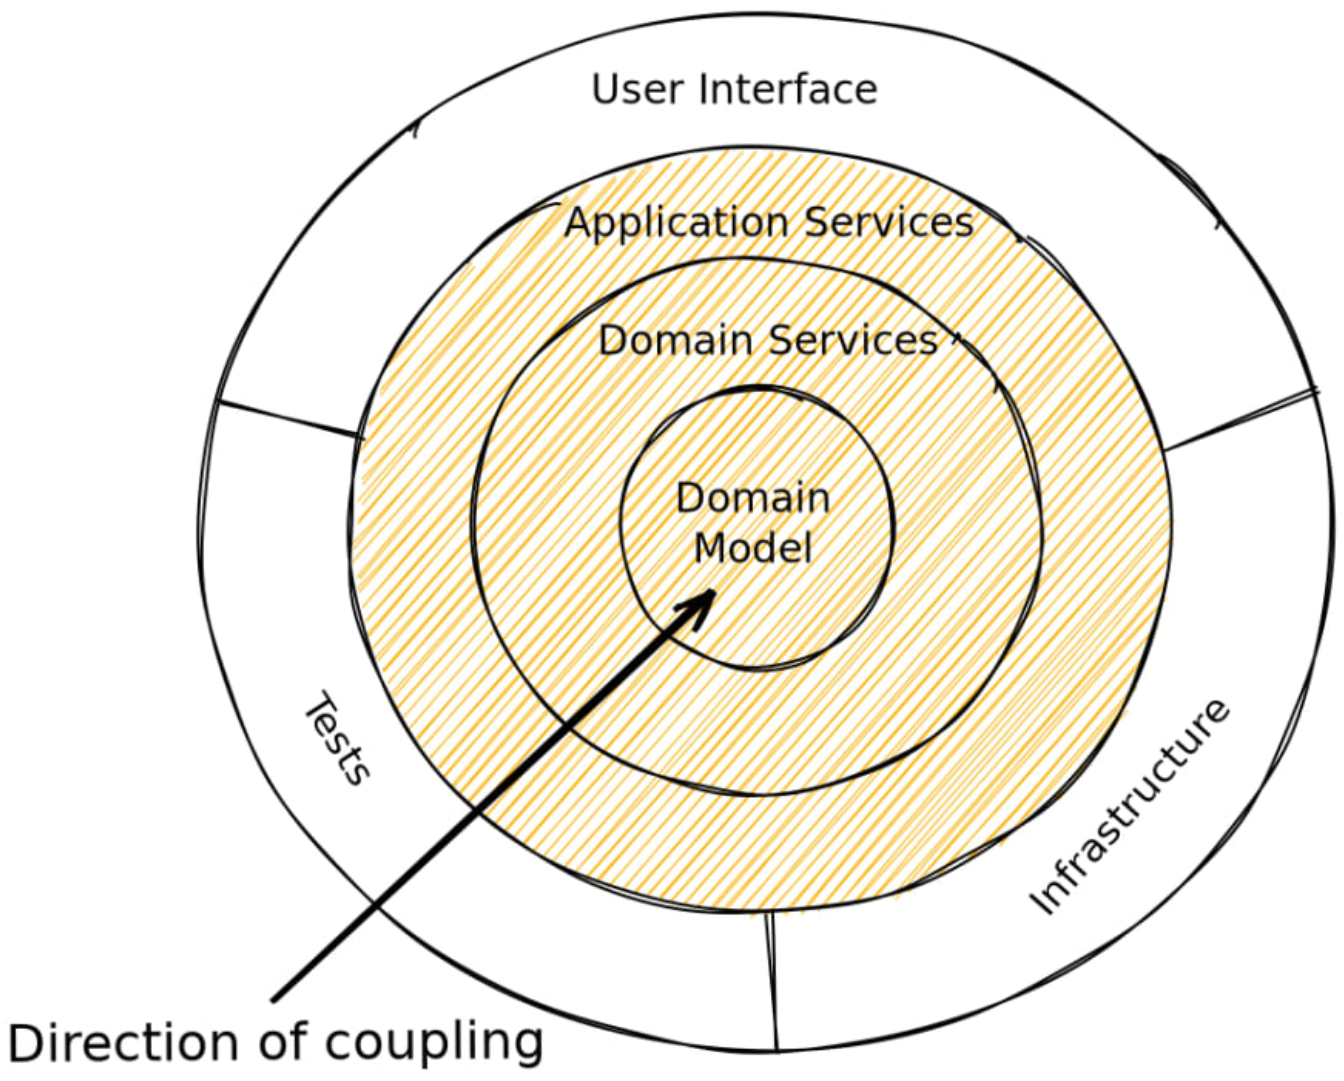
\includegraphics[width=0.8\textwidth]{onionArchitecture.png}
                    \attribution{https://dev.to/barrymcauley/onion-architecture-3fgl}
                \end{center}
            \end{column}
        \end{columns}
    \end{frame}

    \begin{frame}
        \frametitle{Чистая архитектура}
        \begin{center}
            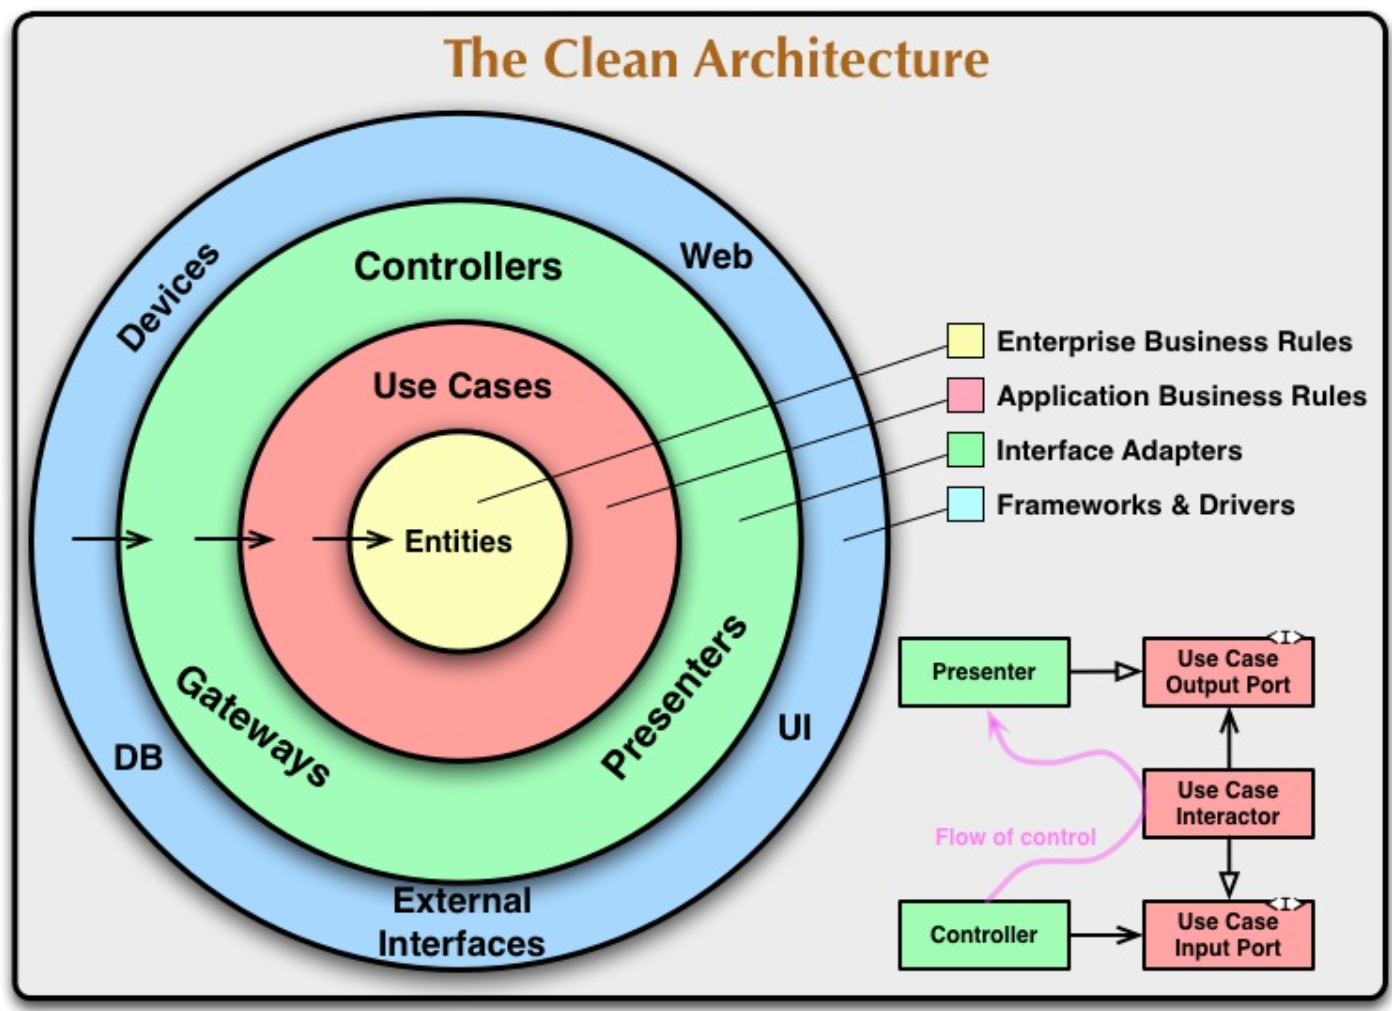
\includegraphics[width=0.6\textwidth]{cleanArchitecture.png}
            \attribution{https://herbertograca.com/2017/09/28/clean-architecture-standing-on-the-shoulders-of-giants/}
        \end{center}
        \begin{itemize}
            \item Дальнейшее развитие луковой --- определяет поток управления
        \end{itemize}
    \end{frame}

    \begin{frame}
        \frametitle{Чистая архитектура, обработка запроса}
        \begin{center}
            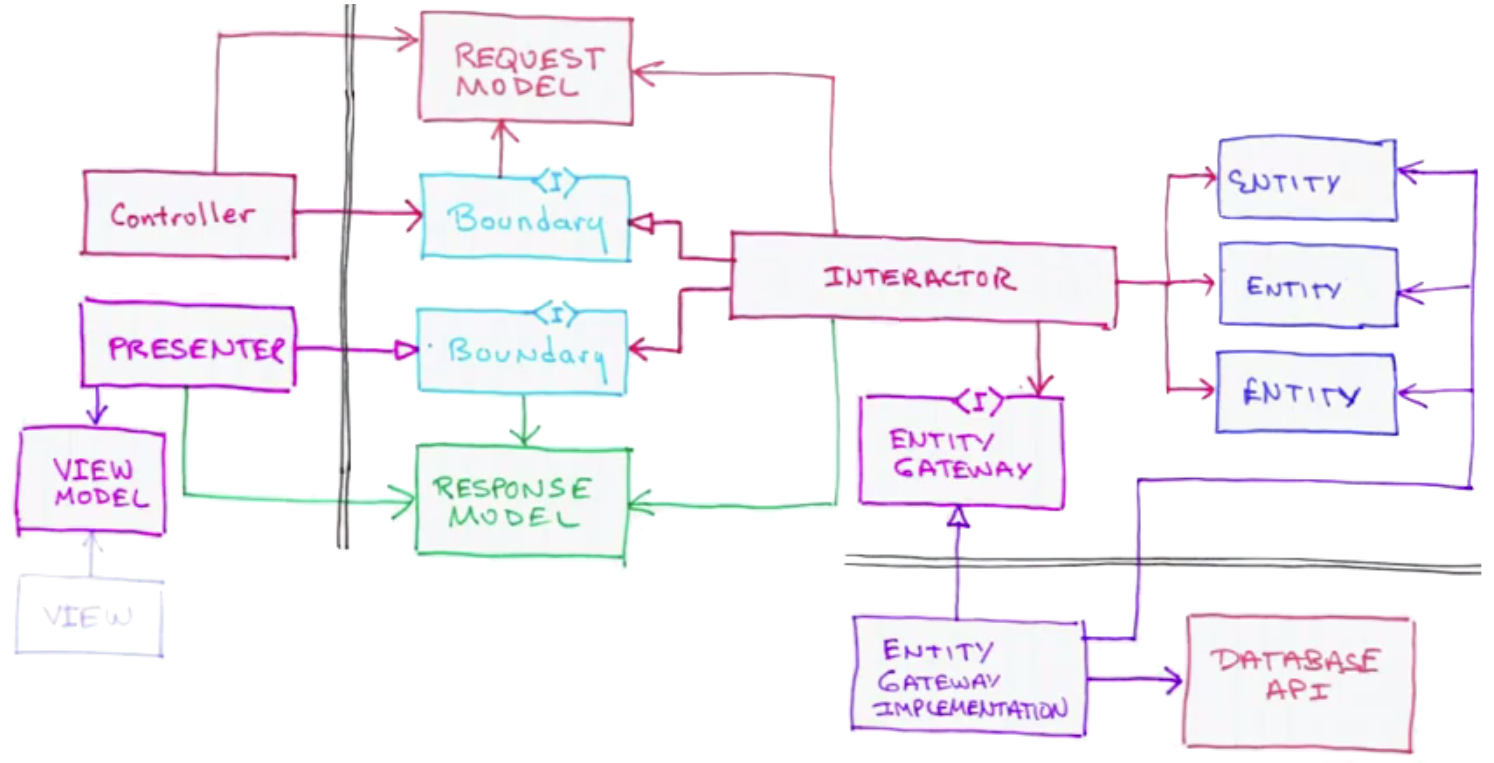
\includegraphics[width=0.8\textwidth]{cleanArchitectureControlFlow.png}
            \attribution{https://herbertograca.com/2017/09/28/clean-architecture-standing-on-the-shoulders-of-giants/}
        \end{center}
    \end{frame}

    \section{REST}

    \begin{frame}
        \frametitle{Дизайн REST-интерфейса}
        \begin{itemize}
            \item API строится вокруг ресурсов, не действий
            \begin{itemize}
                \item \url{http://api.example.com/customers/} --- хорошо
                \item \url{http://api.example.com/get_customer/} --- плохо
            \end{itemize}
            \item Отношения между сущностями: \url{http://api.example.com/customers/5/orders}
            \begin{itemize}
                \item Максимум одно отношение --- надо будет, сделают ещё запросы
            \end{itemize}
            \item API --- модель предметной области, не данных
            \item Семантика HTTP
            \begin{itemize}
                \item Заголовки Content-Type, Accept
                \item Коды возврата (200, 204, 404, 400, 409)
            \end{itemize}
            \item Механизмы фильтрации и <<пагинации>>
            \item Поддержка Partial Content
            \item Hypertext as the Engine of Application State (HATEOAS)
            \item Версионирование --- не ломать обратную совместимость
        \end{itemize}
    \end{frame}

    \section{Общие принципы дизайна}

    \begin{frame}
        \frametitle{Общие принципы дизайна распределённых приложений}
        \framesubtitle{Самовосстановление}
        \begin{itemize}
            \item Повтор при временном отказе
            \item API для самодиагностики
            \item Разделение на изолированные группы ресурсов
            \item Буферизация запросов
            \item Автоматическое переключение на резервный экземпляр, ручное обратно
            \item Промежуточное сохранение
            \item Плавная потеря работоспособности (graceful degradation)
            \item Тестирование отказов, Chaos engineering
        \end{itemize}
    \end{frame}

    \begin{frame}
        \frametitle{Circuit Breaker, поведение}
        \begin{center}
            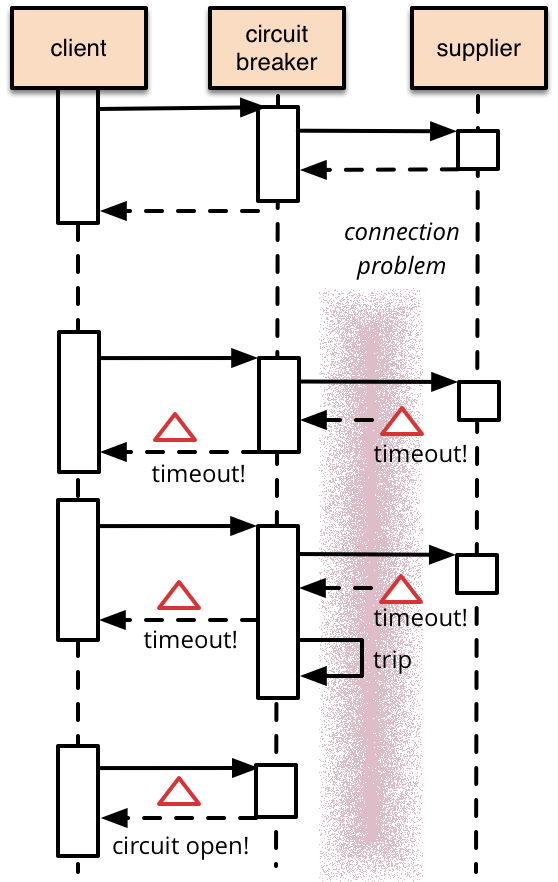
\includegraphics[height=0.7\textheight]{circuitBreakerSequence.png}
            \attribution{\url{https://martinfowler.com/bliki/CircuitBreaker.html}}
        \end{center}
    \end{frame}

    \begin{frame}
        \frametitle{Circuit Breaker, состояния}
        \begin{center}
            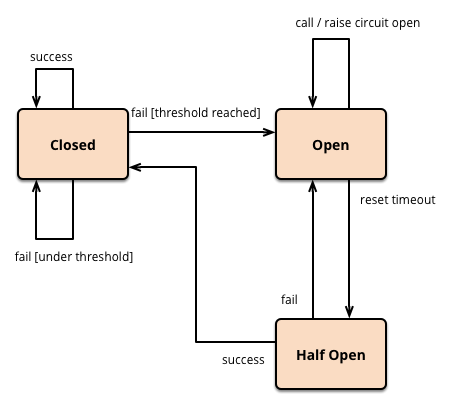
\includegraphics[width=0.5\textwidth]{circuitBreakerStates.png}
            \attribution{\url{https://martinfowler.com/bliki/CircuitBreaker.html}}
        \end{center}
    \end{frame}

    \begin{frame}
        \frametitle{Избыточность}
        \begin{columns}
            \begin{column}{0.5\textwidth}
                \begin{itemize}
                    \item Бизнес-требования к надёжности
                    \begin{itemize}
                        \item Recovery Time Objective, Recovery Point Objective, Maximum Tolerable Outage
                    \end{itemize}
                    \item Балансировщики нагрузки
                    \item Репликация БД
                    \item Разделение по регионам
                    \item Шардирование
                \end{itemize}
            \end{column}
            \begin{column}{0.5\textwidth}
                \begin{center}
                    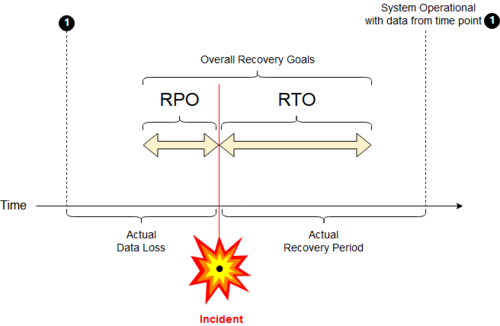
\includegraphics[width=\textwidth]{rpoRtoExample.png}
                    \attribution{\url{https://en.wikipedia.org/wiki/Disaster_recovery}}
                \end{center}
            \end{column}
        \end{columns}
    \end{frame}

    \begin{frame}
        \frametitle{Минимизация координации}
        \begin{itemize}
            \item Доменные события (domain events)
            \item Event Sourcing
            \item Асинхронные, идемпотентные операции
            \item Шардирование
            \item Eventual Consistency, компенсационные транзакции
        \end{itemize}
    \end{frame}

    \begin{frame}
        \frametitle{Command and Query Responsibility Segregation}
        \begin{center}
            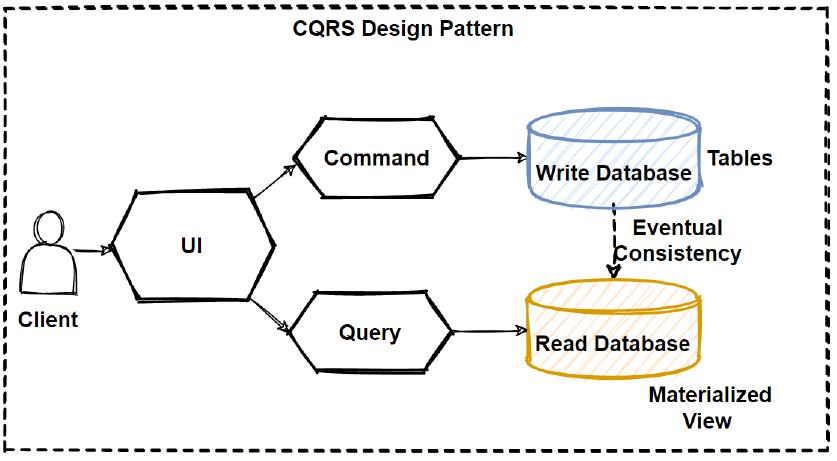
\includegraphics[width=0.8\textwidth]{cqrs.png}
            \attribution{\url{https://medium.com/design-microservices-architecture-with-patterns/cqrs-design-pattern-in-microservices-architectures-5d41e359768c}}
        \end{center}
    \end{frame}

    \begin{frame}
        \frametitle{Проектирование для обслуживания}
        \begin{itemize}
            \item Делать всё наблюдаемым
            \begin{itemize}
                \item Трассировка, в т.ч. распределённая
                \item Логирование 
            \end{itemize}
            \item Мониторинг, метрики
            \item Стандартизация форматов логов и метрик
            \item Автоматизация задач обслуживания
            \item Конфигурация --- это код
        \end{itemize}
    \end{frame}

\end{document}
